\hypertarget{prototyp}{%
\section{Der Prototyp}\label{prototyp}}

\hypertarget{konzeption}{%
\subsection{Konzeption}\label{konzeption}}

\hypertarget{idee}{%
\subsubsection{Idee}\label{idee}}

Aus dem Visionsvideo soll nun ein Prototyp entwickelt werden, der einen
ersten Schritt in Richtung Realisierung der Vision darstellen soll.

Selbstverständlich sind Hologramm-Technologien, wie sie im Video gezeigt
werden, noch längst nicht umsetzbar. Allerdings gibt es heute schon
Möglichkeiten virtuelle Objekte in die reale Welt zu setzen und zwar in
Form von Augmented Reality.

Der Aspekt, dass die Anwendung auf so ziemlich jedem Gerät laufen soll,
lässt sich realisieren: Der Prototyp wird eine Web-Anwendung. Dadurch
geht allerdings auch ein Aspekt verloren: Man kann dem Nutzer keine
Erinnerungen/Notifications schicken, wenn er sich nicht auf der Webseite
befindet. Diese Einschränkung nimmt das Team für den Prototypen aber in
Kauf.

Das Erkennen von Pflanzen und ihrem Zustand anhand von Scans bzw.
Bildern ist zwar prinzipiell möglich, allerdings sind solche
Analysesysteme sehr aufwendig und brauchen sehr viele Testdaten, um
richtig funktionieren zu können. Das würde den Projektrahmen sprengen.
Daher wird der Prototyp nur mit einem Anzuchtkasten umgesetzt, in den
zusätzlich Sensoren eingebaut werden.

Zusammengefasst soll also eine AR-Anwendung im Webbrowser realisiert
werden, die mit einem Anzuchtkasten funktioniert. In den Anzuchtkasten
werden Sensoren eingebaut, die den Zustand im Kasten erfassen. Über
mobile Endgeräte erfolgt nun die Überlagerung von virtuellen Objekten in
die reale Welt, gestützt durch die Messwerte der Sensoren.

\hypertarget{design}{%
\subsubsection{Design}\label{design}}

Das daraus abgeleitete Design findet sich in der Grafik wieder.
Alternativ befindet es sich ebenfalls im
\protect\hyperlink{anhang}{Anhang}.

\begin{figure}
\centering
\includegraphics{img/AblaufVisualisierung_kompr.jpg}
\caption{Grafik - Ablauf und Visualisierung}
\end{figure}

Die Messdaten der Sensoren werden unterschieden in
\textbf{übergreifende} und \textbf{spezifische} Messdaten.
Luftfeuchtigkeit, Belichtung und Temperatur gelten für alle Pflanzen im
Kasten gleich, darum werden sie auch in der Darstellung an den Kasten
angehängt und direkt im Startmenü angezeigt. Lediglich die
Bodenfeuchtigkeit gilt spezifisch für jeden Topf einzeln, der User muss
diesen Topf also zunächst im Startmenü auswählen, um sich dessen gesamte
Daten unter der Menüoption ``Standortdaten'' anzeigen zu lassen.

Außerdem unterschieden werden muss zwischen einem leeren und einem
bepflanzten Topf. Je nachdem wie diese Zustandseigenschaft des Topfes
belegt ist, ergeben sich bei der Auswahl dessen nämlich auch weitere zu
unterscheidende Menü- und Aktivitäts-Optionen. Diese lassen sich der
Ablauf-Grafik entnehmen.

Übergreifende Messdaten werden über dem Kasten als türkise Buttons
dargestellt. Durch Antippen wird zum jeweiligen Messwert ein Diagramm
angezeigt, welches den Verlauf über die letzten Tage visualisiert.

Umfangreichere Inhalte wie Informationen zu einer Pflanze oder auch die
Diagramme werden in einem weißen Popup dargestellt, welches sich auf den
Bildschirm legt und die AR-Szene überdeckt. Das Popup ist am Bildschirm
fest und nicht am Kasten. Er ist scrollbar und kann über ein X
geschlossen werden.

Wichtige Notifications, welche in der Grafik rot dargestellte Symbole
sind, erscheinen, falls ein nötiger Handlungsbedarf besteht (z.B. wenn
die Erde der Pflanze zu trocken ist), am jeweiligen Topf. Durch Antippen
sollen diese direkt zu einer entsprechenden Popup-Nachricht führen und
zu der erforderlichen Aktion im Menü navigieren.

Popup-Nachrichten sind immer unten zu sehen in Form von Sprechblasen,
die von PLANT-E ``gesprochen'' werden. Diese Popup-Nachrichten sollen
auch die Anweisungen z.B. für das Eintopfen darstellen. Dies soll die
Kommunikation von PLANT-E mit dem Nutzer visualisieren.

\hypertarget{architektur}{%
\subsection{Architektur}\label{architektur}}

Aus diesen Anforderungen ist eine Architektur entstanden, die aus drei
Kernkomponenten besteht:

\begin{itemize}
\tightlist
\item
  dem Sensorenhandling über einen Raspberry Pi,
\item
  der Datenverwaltung und Auslieferung der Webseite über einen
  Backend-Server und
\item
  die eigentliche Webseite, die von den Clients aufgerufen wird.
\end{itemize}

Zur Übersicht ist ebenfalls ein Diagramm erstellt worden, welches die
Komponenten und ihr Zusammenspiel verdeutlicht.

\begin{figure}
\centering
\includegraphics{}
\caption{Grafik der Architektur}
\end{figure}

Die Sensordaten werden stetig gemessen und vom Raspberry Pi über
UDP-Pakete an das Backend gesendet. UDP ist ein verbindungsloses
Protokoll. Es werden lediglich Zieladresse und -port angegeben und schon
wird das Datenpaket versendet. Es findet keine Empfangsbestätigung
statt. Die Pakete sind immer kleine abgeschlossene Einheiten. Die Idee
ist, dass die Sensordaten in einem langen konstanten Datenstrom
ausgeliefert werden, egal ob jemand diese Daten entgegennimmt oder
nicht. Die Vorstellung eines Radiosenders ist ein geeigneter Vergleich.
Der Vorteil dieses Vorgehens ist, dass stetig und sehr schnell Daten zur
Verfügung stehen mit geringstem Overhead.

Der Backend-Server ist das Bindeglied für alle Komponenten. Er nimmt den
UDP-Datenstrom des Raspberry Pis entgegen und verarbeitet diese Daten.
Zum Einen werden sie für die Erfassung eines historischen Verlaufes
gespeichert. Zum Anderen können die Daten vom Frontend nun abgerufen
werden. Das Backend liefert immer die aktuellensten erhaltenen Daten
aus. Bricht der Datenstrom vom Raspberry Pi ab, sind immer noch die
zuletzt empfangenen Daten abrufbar.

Zusätzlich liefert das Backend auch die Frontend-Webseite mit allen
zugehörigen Dateien aus. Darüber hinaus stellt das Backend eine REST-API
zur Verfügung, die vom Frontend genutzt werden kann, um Daten abzurufen
und zu senden. Die Speicherung von zusätzlichen Daten, z.B. ob ein Topf
bepflanzt ist und wie lange schon, wird ebenfalls im Backend gespeichert
und verwaltet. Das Backend liefert auch einen Pflanzenkatalog mit den
unterstützen Pflanzenarten aus.

Das Frontend ist eine Webseite, die in jedem modernen Browser aufgerufen
werden kann. Da es sich um eine AR-Anwendung handelt, benötigt der
Client zwingend eine Kamera im Gerät. Die Anwendung ist nur in der Lage
Informationen rund um den Kasten anzuzeigen. Zur Erkennung des Kastens
ist dort ein Marker angebracht dazu -- später mehr.

\hypertarget{umsetzung}{%
\subsection{Umsetzung}\label{umsetzung}}

\hypertarget{raspberry-pi}{%
\subsubsection{Raspberry Pi}\label{raspberry-pi}}

Der Raspberry Pi soll mittels Sensoren verschiedene Daten zu dem
Anzuchtkasten messen und per UDP-Pakete an das Backend senden.

\hypertarget{datenformat}{%
\paragraph{Datenformat}\label{datenformat}}

Die gesendeten UDP-Pakete sollen alle Messdaten im JSON-Format
enthalten. Hier die Spezifikation der zu sendenden Daten:

\begin{verbatim}
{
  "timestamp": 1594639596, // unix timestamp
  "airHumidity": 42, // in Prozent, ganzzahlig
  "light": 123,      // in lux, ganzzahlig
  "temperature": 24, // in Grad, ganzzahlig
  "pots": [ // die Töpfe von links nach rechts
    {
      "soilHumidity": 73, // in Prozent, ganzzahlig
      // "size": 8,       // Höhe der Pflanze in cm
                      // ist nicht umgesetzt worden
    }
  ],
}
\end{verbatim}

Luftfeuchtigkeit, Helligkeit und Temperatur werden für den gesamten
Kasten erfasst. Die Bodenfeuchtigkeit wird für jeden Topf einzeln
gemessen und ausgeliefert. Da der Gruppe nur ein Sensor für die
Bodenfeuchtigkeit zur Verfügung gestellt worden ist, kann der Prototyp
nur einen Topf bedienen.

Die Analyse der Wuchshöhe ist im Verlaufe des Projektes ausgeklammert
worden, da keine geeignete Kamera zur Verfügung gestanden hat. Außerdem
ist die Analyse von Kamerabildern ein recht aufwendiges Verfahren, was
den Rahmen des Projektes gesprengt hätte.

\hypertarget{verwendete-sensoren}{%
\paragraph{Verwendete Sensoren}\label{verwendete-sensoren}}

Zum Verarbeiten der Sensordaten wird ein Raspberry Pi 4 benutzt, da
dieser der Projekt-Gruppe bereits zur Verfügung gestanden hat. Für die
Sensoren ist daher die Auswahl etwas begrenzt gewesen.

\begin{itemize}
\tightlist
\item
  Lichtmessung: \emph{Lichtsensor „BH1750``}

  \begin{itemize}
  \tightlist
  \item
    wandelt bereits auf der Platine die Analogsignale in Digitalsignale
  \end{itemize}
\item
  Messung von Temperatur und Luftfeuchtigkeit: \emph{Sensor „DHT22``}

  \begin{itemize}
  \tightlist
  \item
    wandelt ebenso bereits die Signale, sodass diese ohne zusätzliche
    Bauteile vom Raspberry Pi gelesen werden können
  \end{itemize}
\item
  Messung der Bodenfeuchtigkeit: \emph{„Capacitive Stil Moisture Sensor
  v2.0``}

  \begin{itemize}
  \tightlist
  \item
    wurde von Hardwareexperten der FH empfohlen
  \item
    liefert unter den Feuchtigkeitssensoren wohl die präzisesten Daten
  \end{itemize}
\item
  Signalverarbeitung des Feuchtigkeitssensors: \emph{Analog-Digital
  Wandler „MCP3008``}

  \begin{itemize}
  \tightlist
  \item
    wurde ebenso gewählt aufgrund der Empfehlung führender
    Hardwareexperten der FH
  \end{itemize}
\end{itemize}

Um diese Sensoren auf dem Raspberry Pi nutzen zu können sind externe
Bibliotheken nötig gewesen. Hierbei handelt es sich um:
Adafruit\_ADSx15\footnote{Link:
  \url{https://github.com/adafruit/Adafruit_Python_ADS1x15}},
Adafruit\_DHT\footnote{Link:
  \url{https://github.com/adafruit/Adafruit_Python_DHT}} und
smbus\footnote{Link:
  \url{http://wiki.erazor-zone.de/wiki:linux:python:smbus:doc}}.

\hypertarget{schaltplan}{%
\paragraph{Schaltplan}\label{schaltplan}}

\begin{figure}
\centering
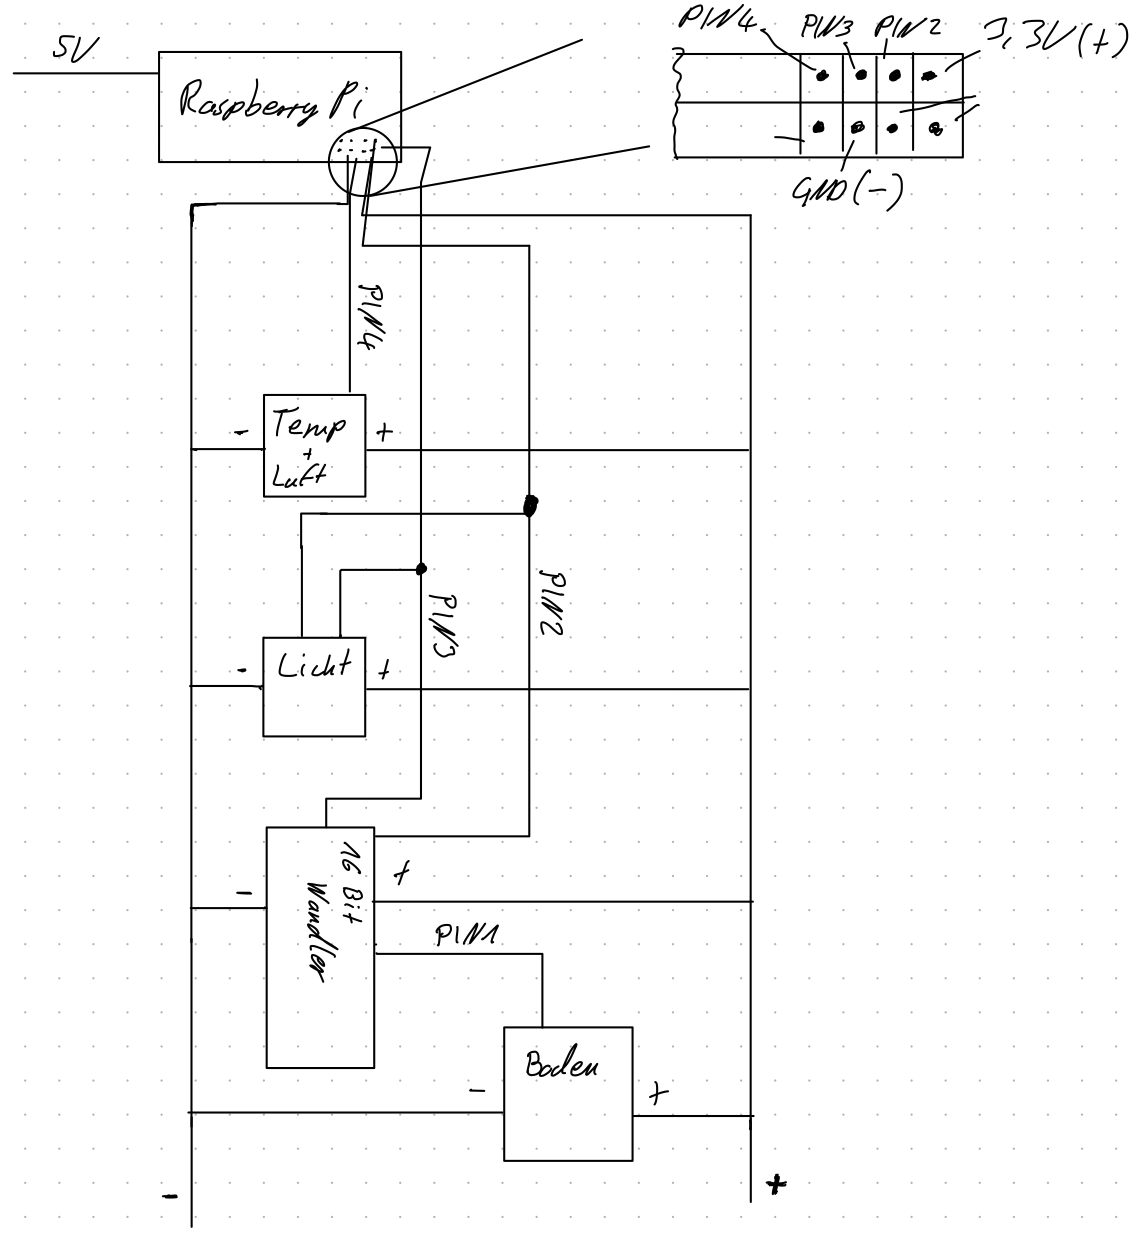
\includegraphics{img/schaltplan.png}
\caption{Schaltplan der Sensoren mit dem Raspberry Pi}
\end{figure}

\hypertarget{skript}{%
\paragraph{Skript}\label{skript}}

Die Anwendung auf dem Raspberry Pi ist als Python-Skript erstellt
worden. Es liest die Sensordaten und versendet sie als UDP-Paket an den
Server.

Es gibt einen Mock-Modus in dem das Skript keine Sensordaten, sondern
Zufallswerte generiert und ausgibt. Das Skript kann dadurch auch auf
einem beliebigen Gerät gestartet werden, liefert dann aber natürlich nur
die Zufallswerte.

\hypertarget{backend}{%
\subsubsection{Backend}\label{backend}}

Das Backend ist ein Node.js-Server, der in TypeScript implementiert
worden ist. Er empfängt zum einen die UDP-Pakete vom Raspberry Pi über
einen entsprechenden Socket. Zum Anderen stellt er einen Express.js
Server zur Verfügung, der sowohl das Frontend inklusive aller benötigten
Dateien ausliefert als auch eine REST-API für das Frontend zur Verfügung
stellt.

Es speichert die Daten vom Raspberry Pi in regelmäßigen Abständen in
einer Historie und speichert auch Daten, die vom Frontend kommen. Zum
Beispiel in welchem Topf sich welche Pflanze befindet und wie lange die
dort schon eingetopft ist usw.

Außerdem liegt ein Katalog mit den unterstützten Pflanzenarten im
Backend vor. Dieser wird verwendet, um die Pflanzendaten anzureichern.

Die Daten werden in JSON-Dateien gespeichert, die beim Start des Servers
geladen werden. Ändern sich die Daten, so werden die Änderungen auch in
die JSON-Dateien geschrieben. Die Verwendung von einem
Datenbanken-System ist für den Prototypen zu aufwendig gewesen.

\hypertarget{frontend}{%
\subsubsection{Frontend}\label{frontend}}

Das Frontend besteht aus einer Webseite, die von der Funktion her eine
SPA (Single-Page-Application) ist. Zum Einsatz kommt das Webframework
\textbf{Vue.js} sowie die Technologien \textbf{AFrame} und
\textbf{AR.js}.

\textbf{Vue.js}\footnote{Link: \url{https://vuejs.org}} ist ein
schlankes Frontend-Framework, welches mit recht simplen HTML-Attributen,
einem Komponenten- und Vorlagensystem das erstellen von interaktiven
Webseiten vereinfacht. Es kann einfach auf die HTML-Struktur
draufgesetzt werden und ist recht leichtgewichtig.

\textbf{AFrame}\footnote{Link: \url{https://aframe.io}} ist ein Wrapper
für Three.js, mittels dem 3D-Modelle in eine Szene gesetzt und gerendert
werden können. AFrame stellt dabei HTML-Tags zur Verfügung, die
3D-Elemente repräsentieren und entsprechend gerendert werden. Der
Mechanismus erfolgt so, dass ein
\texttt{\textless{}a-scene\textgreater{}}-Tag im HTML-Markup gesetzt
werden muss. Diese \texttt{\textless{}a-scene\textgreater{}} wird dann
in ein HTML-Canvas-Element umgewandelt und die 3D-Elemente
(\texttt{\textless{}a-entity\textgreater{}}) innerhalb der
\texttt{\textless{}a-scene\textgreater{}} werden in die Szene gesetzt
und auf den Canvas gemalt. Mit diesem System lassen sich VR-Anwendungen
im Webbrowser darstellen.

\textbf{AR.js}\footnote{Link:
  \url{https://ar-js-org.github.io/AR.js-Docs/}} ist nun eine
Erweiterung für AFrame. Der zugrundeliegende Mechanismus bleibt gleich,
allerdings wird der Hintergrund des Canvas mit dem Bild der
geräteinternen Kamera gefüllt. Zusätzlich kann ein sog. Marker definiert
werden (siehe Bild). Der Marker wird vom Kamerabild erkannt und dient
als Referenzpunkt. Die Position des Markers markiert den Ursprungspunkt
der Szene (Punkt 0,0,0). Die Breite des Markers gibt die Breite von
einer Einheit in AR.js an. Nun können 3D-Elemente relativ zum Marker
platziert werden.

\begin{figure}
\centering

\includegraphics{img/hiro.png}
\caption{Bild des Hiro-Markers von AR.js}
\end{figure}

AR.js funktioniert so, dass die Elemente nur zu sehen sind, wenn auch
der Marker zu sehen ist, zu dem die Elemente ja relativ liegen. Er dient
als Referenz- und Ankerpunkt der Szene. Der Einfachheit halber ist der
Standard-Marker von AR.js verwendet worden.

\hypertarget{ergebnisse-und-herausforderungen}{%
\subsection{Ergebnisse und
Herausforderungen}\label{ergebnisse-und-herausforderungen}}

Die Umsetzung des Raspberry Pi, der Sensoren und des Backends hat sehr
gut funktioniert. Die Daten werden richtig ausgeliefert, im Backend
gespeichert und ausgegeben. Lediglich die Geschwindigkeit der Sensoren
ist nicht optimal. Diese brauchen im Schnitt etwas unter einer Sekunde,
um die Messdaten zu erheben und zu versenden. Dies ist für sehr
interaktive Use-Cases wie zum Beispiel der Gießanzeige zwar unpraktisch,
für den Prototypen ist es aber ausreichend. Hier können in Zukunft
Optimierungen vorgenommen werden, etwa mit besserer Hardware.

Bezüglich des Backends fehlen natürlich reale, über einen längeren
Zeitraum erhobene Daten. Wären diese vorhanden, könnten sich noch neue
Erkenntnisse gewinnen und zum Beispiel eine sehr umfangreiche Historie
mit vielen Optionen und Ansichten erzeugen lassen. Für einen Protoypen
sind die vorhandenen Daten aber ausreichend.

Sehr ernüchternd ist hingegen das Frontend ausgefallen. Die anfängliche
Euphorie über die AR-Technik im Browser ist sehr schnell verflogen, weil
sich sehr bald gravierende Schwierigkeiten ergeben haben. Der
Projektfortschritt ist dadurch so stark behindert worden, dass nur ein
Bruchteil der geplanten Funktionalität überhaupt umgesetzt werden
konnte.

Ein großes Problem, welches immernoch nicht abschließend gelöst werden
konnte, ist das Anklicken von Elementen in AR.js. Es hat sehr lange
gedauert, bis es überhaupt möglich gewesen ist, auf Klicks zu reagieren.
Das hängt damit zusammen, dass Klicks in der Szene über einen Raycaster
umgesetzt werden. Dieser Raycaster ist in der Standard-Konfiguration zu
langsam. Da im AR-Modus die Szene ständig verschoben wird, aufgrund des
wackelnden Markers durch die wackelige Hand des Nutzers, muss der
Raycaster sehr schnell immer wieder nach Kollisionen checken, ansonsten
werden niemals irgendwelche Klicks erkannt. Diese Erkenntnis zu gewinnen
und das Problem zu lösen, hat alleine 2 Wochen in Anspruch genommen.

Damit nicht genug funktionieren Klicks im AR-Modus nur in der Mitte des
Bildschirms einigermaßen zuverlässig. Weiter am Rand funktionieren sie
so gut wie gar nicht. Die genaue Ursache ist bis heute nicht geklärt
worden. Durch das Wackeln werden zusätzlich manchmal Element angeklickt,
die man gar nicht klicken wollte. Insgesamt ist das Interagieren mit der
AR-Anwendung sehr mühselig und ist alles andere als intuitiv und
ausgereift.

Auch die Erkennung des Markers in AR.js funktioniert nur unter guten
Lichtverhältnissen und freie Sicht der Kamera auf den Marker. Wird der
Marker verloren, so verschwinden einfach alle 3D-Elemente. Dies stellt
keine schöne User Experience dar und ist gerade für die Entwicklung sehr
anstrengend.

Deswegen ist während der Entwicklung der AR-Modus meistens ausgeschaltet
gewesen. Die App wurde hauptsächlich im VR-Modus entwickelt, da hier
nichts wackelt und die Entwickler besser testen können, was sie
eigentlich tun. Daher funktioniert die Anwendung im VR-Modus recht gut,
im AR-Modus eher weniger.

Auch im Design sind die Möglichkeiten von AFrame und AR.js sehr
beschränkt. So ist es nicht möglich zum Beispiel die Ecken von einem
Button abzurunden. Das komplette Design hat eigentlich auf ``Kapseln''
basiert. Da sich dies nicht realisieren lassen hat, sind überall
langgezogene Kreise und Kugeln zum Einsatz gekommen. Das Erstellen oder
Verändern von eigenen Geometrien und Meshes ist schwerlich möglich, da
AFrame dafür keinen Editor oder Oberfläche bietet, wie man es z.B. von
Unity kennt.

Das gravierendste Problem ist das nicht vorhandene Logging von Fehlern
in AFrame und AR.js. Fehler in der Syntax werden nicht angezeigt und
auch beim Auftreten von Fehlern während des Aufrufens der Seite, gibt es
so gut wie keine Logs oder Hinweise. Die Entwickler tappen die ganze
Zeit im Dunkeln und können sich nur durch kleine Änderungen und stetiges
Ausprobieren im Browser langsam voranbewegen. Gibt die Dokumentation von
AFrame wenigstens noch einen guten Überblick, so ist sie für AR.js viel
zu lückenhaft, um damit ordentlich arbeiten zu können. Insgesamt ist die
Entwicklung mit diesen Technologien sehr zäh gewesen und hat alles
andere als zufriedenstellende Ergebnisse produziert.

Das Projekt ist auch durch die Vielzahl an unterschiedlichen Komponenten
sehr komplex gewesen. Dieses Zusammenspiel hat sich aber durch Mocking
und Fake-Daten recht elegant lösen lassen. Trotzdem hat das
beschwerliche Arbeiten im Frontend dazu geführt, dass viele
Funktionalitäten zwar theoretisch über Raspberry Pi und Backend zur
Verfügung stehen, diese aber im Frontend nicht umgesetzt werden konnten.
Tatsächlich sind die Sensoren und das Backend dem Frontend weit voraus.
Dies ist für das Projektteam besonders frustrierend, da ja theoretisch
mehr funktioniert, aber das Frontend nicht in der Lage ist, das
darzustellen.
